\documentclass{article}\usepackage[]{graphicx}\usepackage[]{color}
%% maxwidth is the original width if it is less than linewidth
%% otherwise use linewidth (to make sure the graphics do not exceed the margin)
\makeatletter
\def\maxwidth{ %
  \ifdim\Gin@nat@width>\linewidth
    \linewidth
  \else
    \Gin@nat@width
  \fi
}
\makeatother

\definecolor{fgcolor}{rgb}{0.345, 0.345, 0.345}
\newcommand{\hlnum}[1]{\textcolor[rgb]{0.686,0.059,0.569}{#1}}%
\newcommand{\hlstr}[1]{\textcolor[rgb]{0.192,0.494,0.8}{#1}}%
\newcommand{\hlcom}[1]{\textcolor[rgb]{0.678,0.584,0.686}{\textit{#1}}}%
\newcommand{\hlopt}[1]{\textcolor[rgb]{0,0,0}{#1}}%
\newcommand{\hlstd}[1]{\textcolor[rgb]{0.345,0.345,0.345}{#1}}%
\newcommand{\hlkwa}[1]{\textcolor[rgb]{0.161,0.373,0.58}{\textbf{#1}}}%
\newcommand{\hlkwb}[1]{\textcolor[rgb]{0.69,0.353,0.396}{#1}}%
\newcommand{\hlkwc}[1]{\textcolor[rgb]{0.333,0.667,0.333}{#1}}%
\newcommand{\hlkwd}[1]{\textcolor[rgb]{0.737,0.353,0.396}{\textbf{#1}}}%
\let\hlipl\hlkwb

\usepackage{framed}
\makeatletter
\newenvironment{kframe}{%
 \def\at@end@of@kframe{}%
 \ifinner\ifhmode%
  \def\at@end@of@kframe{\end{minipage}}%
  \begin{minipage}{\columnwidth}%
 \fi\fi%
 \def\FrameCommand##1{\hskip\@totalleftmargin \hskip-\fboxsep
 \colorbox{shadecolor}{##1}\hskip-\fboxsep
     % There is no \\@totalrightmargin, so:
     \hskip-\linewidth \hskip-\@totalleftmargin \hskip\columnwidth}%
 \MakeFramed {\advance\hsize-\width
   \@totalleftmargin\z@ \linewidth\hsize
   \@setminipage}}%
 {\par\unskip\endMakeFramed%
 \at@end@of@kframe}
\makeatother

\definecolor{shadecolor}{rgb}{.97, .97, .97}
\definecolor{messagecolor}{rgb}{0, 0, 0}
\definecolor{warningcolor}{rgb}{1, 0, 1}
\definecolor{errorcolor}{rgb}{1, 0, 0}
\newenvironment{knitrout}{}{} % an empty environment to be redefined in TeX

\usepackage{alltt}

\usepackage{graphicx}
\usepackage{float}
\usepackage{amsmath}
\usepackage{mathtools}
\usepackage{blindtext}
\usepackage[inline]{enumitem}
\usepackage{xcolor}
\usepackage{bm}
\usepackage {fancyvrb}
\usepackage {listings}
\usepackage[makeroom]{cancel}
\IfFileExists{upquote.sty}{\usepackage{upquote}}{}
\begin{document}

\title{Turning Off Atoms in a Two MeOH System}
\maketitle

In this case we have two MeOH molecules separated by 5\AA\ in the $y$ direction.

\begin{figure}[H]
  \center
  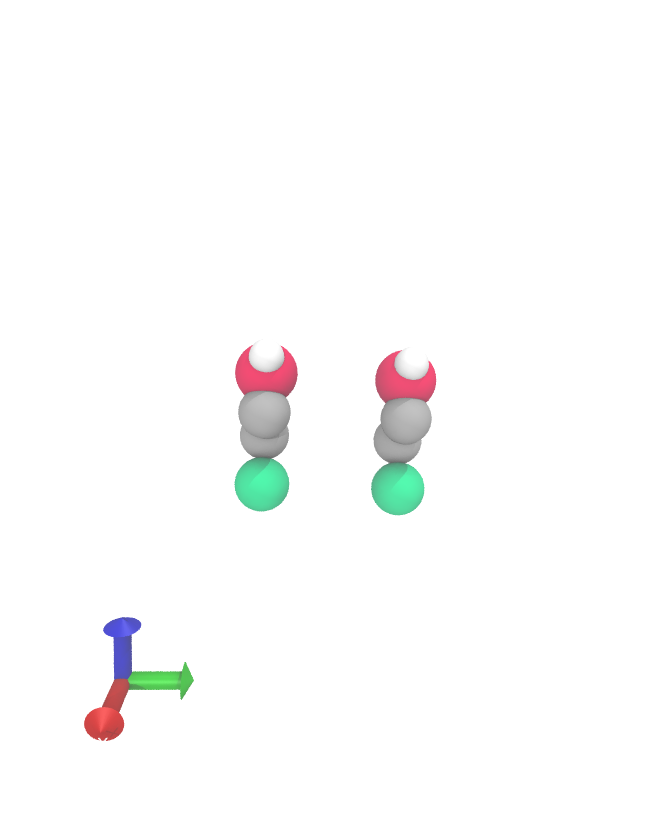
\includegraphics[trim=0 0 0 300,clip,width=0.5\textwidth]{two_meoh}
\end{figure}

Our MeOH molecules have the following coordinates:

\begin{align*}
  &S\ (0.138,0.0,-1.654)   &S'\ (0.138,5.0,-1.654)\\
  &C1\ (0.474,0.0,1.059)   &C1'\ (0.474,5.0,1.059)\\
  &C2\ (-0.621,0.0,-0.007) &C2'\ (-0.621,5.0,-0.007)\\
  &O\ (-0.125,0.0,2.357)   &O'\ (-0.125,5.0,2.357)\\
  &H\ (0.598,0.0,2.999)    &H'\ (0.598,5.0,2.999)\\
\end{align*}

\begin{knitrout}
\definecolor{shadecolor}{rgb}{0.969, 0.969, 0.969}\color{fgcolor}\begin{kframe}
\begin{alltt}
  \hlstd{S}\hlkwb{=}\hlkwd{c}\hlstd{(}\hlnum{2}\hlstd{,}\hlnum{0.0}\hlstd{,}\hlnum{0.138}\hlstd{,}\hlnum{0.0}\hlstd{,}\hlopt{-}\hlnum{1.654}\hlstd{)}
  \hlstd{C1}\hlkwb{=}\hlkwd{c}\hlstd{(}\hlnum{1}\hlstd{,}\hlnum{0.0}\hlstd{,}\hlnum{0.474}\hlstd{,}\hlnum{0.0}\hlstd{,}\hlnum{1.059}\hlstd{)}
  \hlstd{C2}\hlkwb{=}\hlkwd{c}\hlstd{(}\hlnum{1}\hlstd{,}\hlnum{0.265}\hlstd{,}\hlopt{-}\hlnum{0.621}\hlstd{,}\hlnum{0.0}\hlstd{,}\hlopt{-}\hlnum{0.007}\hlstd{)}
  \hlstd{O}\hlkwb{=}\hlkwd{c}\hlstd{(}\hlnum{3}\hlstd{,}\hlopt{-}\hlnum{0.700}\hlstd{,}\hlopt{-}\hlnum{0.125}\hlstd{,}\hlnum{0.0}\hlstd{,}\hlnum{2.357}\hlstd{)}
  \hlstd{H}\hlkwb{=}\hlkwd{c}\hlstd{(}\hlnum{4}\hlstd{,}\hlnum{0.435}\hlstd{,}\hlnum{0.598}\hlstd{,}\hlnum{0.0}\hlstd{,}\hlnum{2.999}\hlstd{)}
  \hlstd{S_2}\hlkwb{=}\hlkwd{c}\hlstd{(}\hlnum{2}\hlstd{,}\hlnum{0.0}\hlstd{,}\hlnum{0.138}\hlstd{,}\hlnum{5.0}\hlstd{,}\hlopt{-}\hlnum{1.654}\hlstd{)}
  \hlstd{C1_2}\hlkwb{=}\hlkwd{c}\hlstd{(}\hlnum{1}\hlstd{,}\hlnum{0.0}\hlstd{,}\hlnum{0.474}\hlstd{,}\hlnum{5.0}\hlstd{,}\hlnum{1.059}\hlstd{)}
  \hlstd{C2_2}\hlkwb{=}\hlkwd{c}\hlstd{(}\hlnum{1}\hlstd{,}\hlnum{0.265}\hlstd{,}\hlopt{-}\hlnum{0.621}\hlstd{,}\hlnum{5.0}\hlstd{,}\hlopt{-}\hlnum{0.007}\hlstd{)}
  \hlstd{O_2}\hlkwb{=}\hlkwd{c}\hlstd{(}\hlnum{3}\hlstd{,}\hlopt{-}\hlnum{0.700}\hlstd{,}\hlopt{-}\hlnum{0.125}\hlstd{,}\hlnum{5.0}\hlstd{,}\hlnum{2.357}\hlstd{)}
  \hlstd{H_2}\hlkwb{=}\hlkwd{c}\hlstd{(}\hlnum{4}\hlstd{,}\hlnum{0.435}\hlstd{,}\hlnum{0.598}\hlstd{,}\hlnum{5.0}\hlstd{,}\hlnum{2.999}\hlstd{)}
\end{alltt}
\end{kframe}
\end{knitrout}

If we turn off 1 atom then we now have 9 atoms this gives a total number of combinations of:

\[\binom{9}{2}-\binom{4}{2}-\binom{5}{2}+2=22 \]


The LJ Parameters are:

% latex table generated in R 3.3.3 by xtable 1.8-2 package
% Wed May 10 10:36:18 2017
\begin{table}[ht]
\centering
\begin{tabular}{|l||c||c|}
  \hline
Elements & Epsilons (kcal/mol) & Sigmas (A) \\ 
  \hline
C & 0.118 & 3.905 \\ 
  S & 0.397 & 4.250 \\ 
  O & 0.200 & 2.850 \\ 
  H & 0.000 & 1.780 \\ 
   \hline
\end{tabular}
\end{table}


\section{Turning off one $H$ atom}

Calculating the energies of all possible combinations when we turn off a hydrogen atom ($H$) we get:

\begin{knitrout}
\definecolor{shadecolor}{rgb}{0.969, 0.969, 0.969}\color{fgcolor}\begin{kframe}
\begin{alltt}
  \hlstd{distance}\hlkwb{=}\hlkwa{function}\hlstd{(}\hlkwc{atom1}\hlstd{,}\hlkwc{atom2}\hlstd{)\{}
    \hlkwd{return}\hlstd{(}\hlkwd{norm}\hlstd{(atom1[}\hlnum{3}\hlopt{:}\hlnum{5}\hlstd{]}\hlopt{-}\hlstd{atom2[}\hlnum{3}\hlopt{:}\hlnum{5}\hlstd{],}\hlkwc{type}\hlstd{=}\hlstr{"2"}\hlstd{))}
  \hlstd{\}}
  \hlstd{energy}\hlkwb{=}\hlkwa{function}\hlstd{(}\hlkwc{atom1}\hlstd{,}\hlkwc{atom2}\hlstd{)\{}
    \hlstd{r}\hlkwb{=}\hlkwd{distance}\hlstd{(atom1,atom2)}
    \hlstd{sigma} \hlkwb{=} \hlstd{(sigmas[atom1[}\hlnum{1}\hlstd{]]}\hlopt{+}\hlstd{sigmas[atom2[}\hlnum{1}\hlstd{]])}\hlopt{/}\hlnum{2}
    \hlstd{epsilon} \hlkwb{=} \hlkwd{sqrt}\hlstd{(epsilons[atom1[}\hlnum{1}\hlstd{]]}\hlopt{*}\hlstd{epsilons[atom2[}\hlnum{1}\hlstd{]])}
    \hlkwd{return}\hlstd{(}\hlnum{4}\hlopt{*}\hlstd{epsilon}\hlopt{*}\hlstd{((sigma}\hlopt{/}\hlstd{r)}\hlopt{^}\hlnum{12}\hlopt{-}\hlstd{(sigma}\hlopt{/}\hlstd{r)}\hlopt{^}\hlnum{6}\hlstd{))}
  \hlstd{\}}
  \hlstd{atoms} \hlkwb{=} \hlkwd{list}\hlstd{(S,C1,C2,O,S_2,C1_2,C2_2,O_2,H_2)}
  \hlstd{atom_combos} \hlkwb{=} \hlkwd{combn}\hlstd{(atoms,}\hlnum{2}\hlstd{)}
  \hlstd{distances}\hlkwb{=}\hlkwd{mapply}\hlstd{(distance,atom_combos[}\hlnum{1}\hlstd{,],atom_combos[}\hlnum{2}\hlstd{,])}
  \hlstd{interm_energies} \hlkwb{=} \hlkwd{mapply}\hlstd{(energy,atom_combos[,distances}\hlopt{>=}\hlnum{5}\hlstd{][}\hlnum{1}\hlstd{,],atom_combos[,distances}\hlopt{>=}\hlnum{5}\hlstd{][}\hlnum{2}\hlstd{,])}
  \hlkwd{sprintf}\hlstd{(}\hlstr{"Total intermolecular Van der Waals Energy is: %4.4f kcal/mol"}\hlstd{,}\hlkwd{sum}\hlstd{(interm_energies))}
\end{alltt}
\begin{verbatim}
## [1] "Total intermolecular Van der Waals Energy is: -1.3899 kcal/mol"
\end{verbatim}
\end{kframe}
\end{knitrout}

Adding in the intramolecular energy of $-0.2812$ we get a total Van der Waals energy of:

$$\boxed{\text{Total Van der Waals Energy}=-1.3898847+-0.2812=-1.6710847\ \text{kcal/mol}}$$

The total coulombic energy when we turn off 1 hydrogen atom is:

\begin{knitrout}
\definecolor{shadecolor}{rgb}{0.969, 0.969, 0.969}\color{fgcolor}\begin{kframe}
\begin{alltt}
  \hlstd{coul_energy}\hlkwb{=}\hlkwa{function}\hlstd{(}\hlkwc{atom1}\hlstd{,}\hlkwc{atom2}\hlstd{)\{}
    \hlstd{r}\hlkwb{=}\hlkwd{distance}\hlstd{(atom1,atom2)}
    \hlstd{k}\hlkwb{=}\hlnum{0.2}
    \hlkwd{return}\hlstd{(}\hlnum{332.0636}\hlopt{*}\hlstd{((atom1[}\hlnum{2}\hlstd{]}\hlopt{*}\hlstd{atom2[}\hlnum{2}\hlstd{])}\hlopt{/}\hlstd{r)}\hlopt{*}\hlkwd{exp}\hlstd{(}\hlopt{-}\hlstd{k}\hlopt{*}\hlstd{r))}
  \hlstd{\}}
  \hlstd{charged_atoms} \hlkwb{=} \hlkwd{list}\hlstd{(C2,O,C2_2,O_2,H_2)}
  \hlstd{charge_combos} \hlkwb{=} \hlkwd{combn}\hlstd{(charged_atoms,}\hlnum{2}\hlstd{)}
  \hlstd{distances}\hlkwb{=}\hlkwd{mapply}\hlstd{(distance,charge_combos[}\hlnum{1}\hlstd{,],charge_combos[}\hlnum{2}\hlstd{,])}
  \hlkwd{print}\hlstd{(distances)}
\end{alltt}
\begin{verbatim}
##  [1] 2.4154735 5.0000000 5.5528832 5.9600333 5.5528832 5.0000000 5.0926312
##  [8] 2.4154735 3.2437628 0.9668987
\end{verbatim}
\begin{alltt}
  \hlstd{interm_energies} \hlkwb{=} \hlkwd{mapply}\hlstd{(coul_energy,charge_combos[,distances}\hlopt{>=}\hlnum{5}\hlstd{][}\hlnum{1}\hlstd{,],charge_combos[,distances}\hlopt{>=}\hlnum{5}\hlstd{][}\hlnum{2}\hlstd{,])}
  \hlkwd{print}\hlstd{(}\hlkwd{sum}\hlstd{(interm_energies))}
\end{alltt}
\begin{verbatim}
## [1] 1.159854
\end{verbatim}
\end{kframe}
\end{knitrout}

The coulombic energy calculated here is:

\begin{align*}
  \Aboxed{\text{Total Coulombic Energy}=1.1598538\ \text{kcal/mol}}
\end{align*}

\end{document}
